Las mediciones fueron realizadas sobre un amplificador realimentado que se encontraba preparado en el Laboratorio de Electrónica, presentado en la sección \ref{sec:Amp2}. 

%Este amplificador cuenta con 4 resistencias a las salida de diferentes valores, las cuales se pueden seleccionar con un jumper para que sea nuestra carga. 

Para este experimento se realizó la siguiente conexión para comenzar con las mediciones.

\begin{figure}[H]
    \centering
    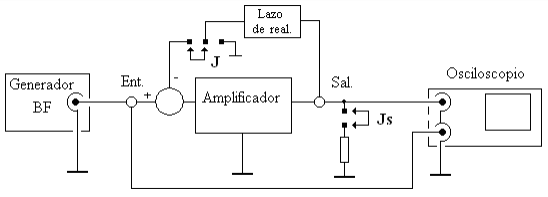
\includegraphics[width=0.9\textwidth]{Imagenes/conexion_p5.png}
    \caption{Esquema de medición}
    \label{fig:esq_conexion}
\end{figure}

En primer lugar se realizaron las mediciones a lazo abierto y sin carga, por lo tanto el jumper \textbf{J} se conecto entre 2 y 3; y el jumper \textbf{Js} se deja desconectado. En estas condiciones se configuró el generador de funciones para introducir en la entrada una señal sinusoidal de 1 kHz y  se ajusto el nivel, de manera que la forma de onda de salida tenga la máxima amplitud libre de distorsión por recorte.

Con el osciloscopio se midió la tensión de la señal de salida y de la señal de entrada (figura \ref{fig:amp2LA}), para así, obtener el valor de la ganancia a lazo abierto. 

\begin{figure}[H]
    \centering
    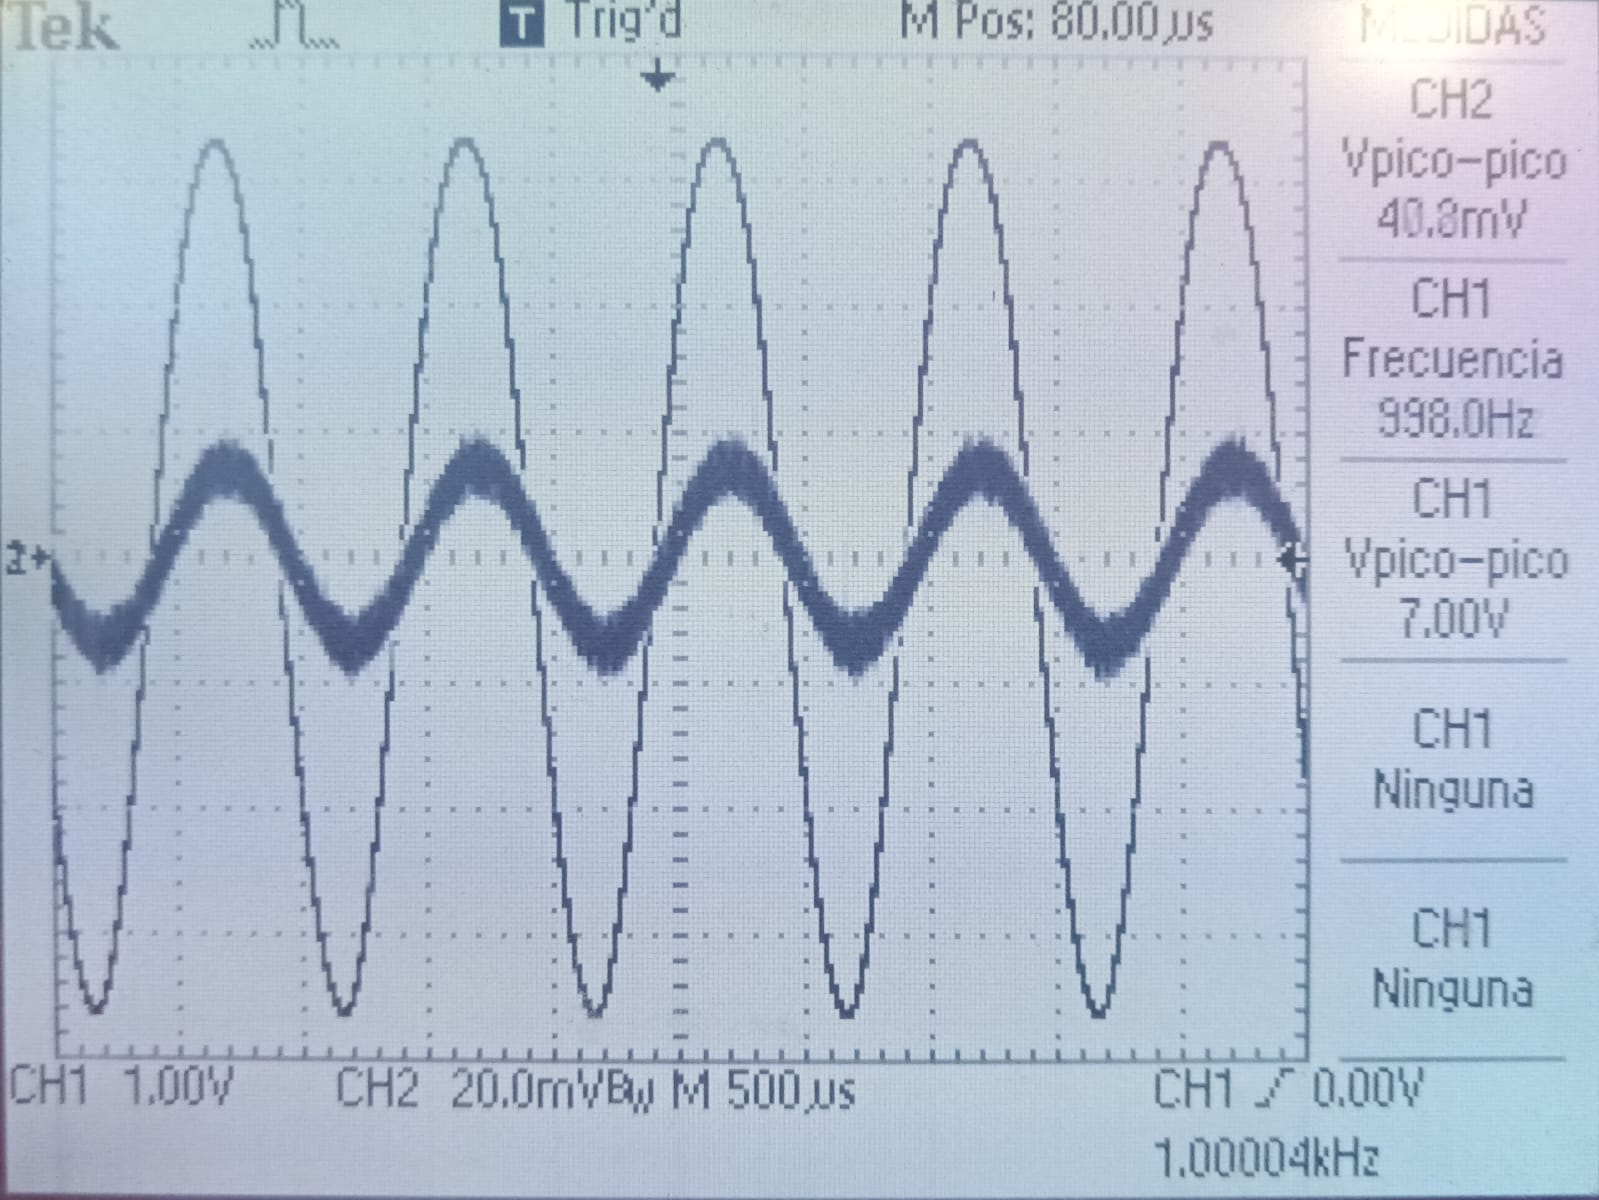
\includegraphics[width=0.6\textwidth]{Imagenes/Amp2LA.jpeg}
    \caption{Señal de entrada y salida, a lazo abierto}
    \label{fig:amp2LA}
\end{figure}

Los datos medidos y calculados se pueden apreciar en la tabla \ref{tab:exp5}.

\begin{table}[H]
    \centering
    \scalebox{1}{
    \begin{tabular}{|c|c|c|}
    \hline
         $V_i$ [$mV_{pp}$] & $V_o$ [$V_{pp}$] & $A=\cfrac{V_o}{V_i}$  [\ohm] \\
    \hline
        40  & 7  & 175\\
    \hline
        \end{tabular}}
        \def\tablename{Tabla} 
        \caption{Valores medidos de tensión y ganancia calculada}
        \label{tab:exp5}
\end{table}

Luego, se procedió a conectar la resistencia de 1 k\ohm ~como resistencia de carga mediante el jumper \textit{JS}, y se procedió a medir nuevamente la tensión de salida. 

Con estos valores de tensión en vacío y con una carga conectada, es posible mediante un cálculo, obtener el valor de resistencia de salida \textit{Ro} del amplificador. A continuación, se presentan los datos en la tabla \ref{tab1:exp5b}.

\begin{table}[H]
    \centering
    \scalebox{1}{
    \begin{tabular}{|c|c|c|}
    \hline
         $V_o$ [$V_{pp}$] & $V_s$ [$V_{pp}$] & $R_o= R_l \cdot (\cfrac{V_o}{V_s}-1)$ [\ohm]\\
    \hline
        7  & 4,52 & 548,67 \\
    \hline
        \end{tabular}}
        \def\tablename{Tabla} 
        \caption{Valores de tensión medidos y resistencia calculada}
        \label{tab1:exp5b}
\end{table}


Una vez obtenido las mediciones a lazo abierto, se conectó el jumper \textit{J} entre 1 y 2, cerrando el lazo, y se realizaron nuevamente los mismos pasos que anteriormente, se desconectó la carga y se configuró la amplitud del generador para obtener la máxima tensión de entrada que no recorte la señal de salida. Una vez todo configurado se volvieron a efectuar las mediciones (figura \ref{fig:amp2LC}) pero ahora, en condición de realimentación (tabla \ref{tab:exp5c}). 

\begin{figure}[H]
    \centering
    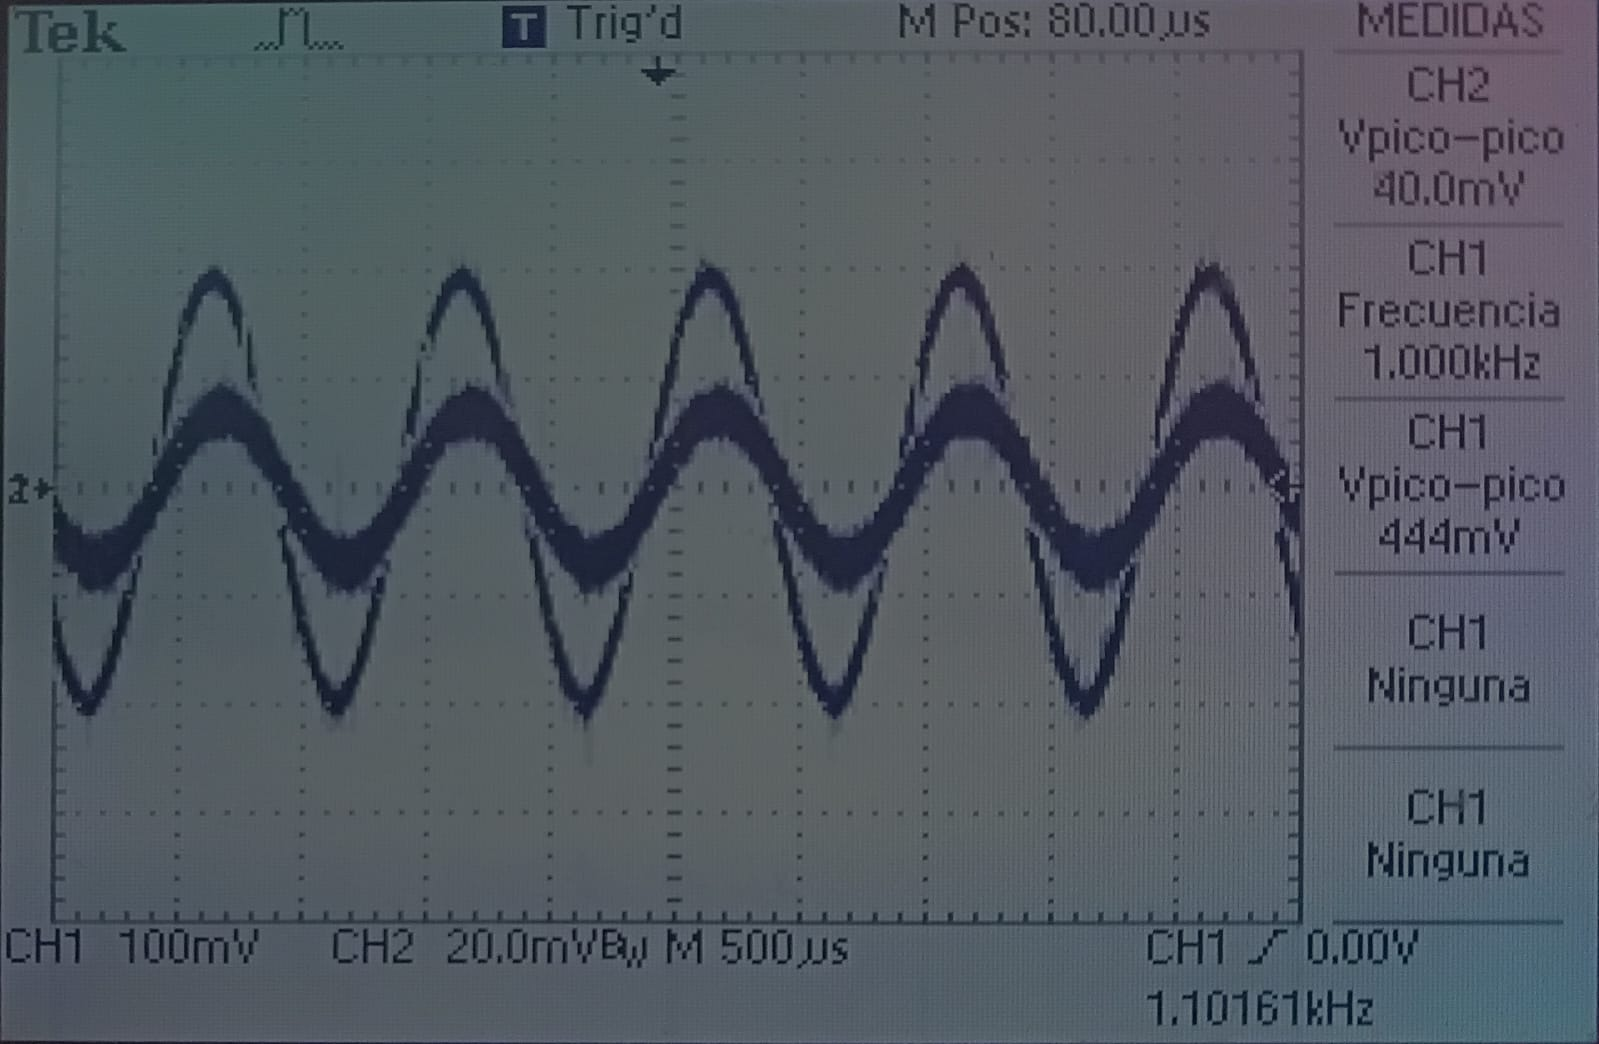
\includegraphics[width=0.6\textwidth]{Imagenes/Amp2LC.jpeg}
    \caption{Señal de entrada y salida, a lazo cerrado}
    \label{fig:amp2LC}
\end{figure}


\begin{table}[H]
    \centering
    \scalebox{1}{
    \begin{tabular}{|c|c|c|}
    \hline
         $V_i$ [$mV_{pp}$] & $V_o$'[$mV_{pp}$] & $G=\cfrac{V_o'}{V_i}$ \\
    \hline
        40  & 444 & 11,1\\
    \hline
        \end{tabular}}
        \def\tablename{Tabla} 
        \caption{Valores medidos de tensión y ganancia calculada}
        \label{tab:exp5c}
\end{table}

Con los valores de tensión de entrada y salida y la ganancia a lazo cerrado ya es posible obtener el valor de resistencia de salida del circuito con realimentación \textbf{$R_0'$} utilizando la siguiente fórmula (ecuación \ref{eq:Rop}):

\begin{equation}
     R_0'= \frac{R_o \cdot G}{A}= \cfrac{548,67 [\ohm] \cdot 11,1}{175}= 34,8~\ohm
     \label{eq:Rop}
\end{equation}

Otra forma de  obtener la Resistencia de salida a lazo cerrado \textbf{Ro'}, es midiendo la tensión de salida con una carga conectada, esta resistencia debe ser de un valor bajo. En el amplificador en cuestión hay dos valores que se pueden usar, una de 100\ohm y una de 33\ohm. 

Para comprobar cuánta variación producía el usar una u otra resistencia, de realizaron las mediciones con las dos resistencias obteniendo los siguientes valores:

\vspace{0.5cm}
\textbf{Con $R_l$= 100~\ohm}:

\begin{table}[H]
    \centering
    \scalebox{1}{
    \begin{tabular}{|c|c|c|}
    \hline
         $V_o$ [$mV_{pp}$] & $V_s$ [$mV_{pp}]$ & $R_o' = R_l \cdot (\cfrac{V_o}{V_s}-1)$ [\ohm]\\
    \hline
        444  & 300 & 48 \\
    \hline
        \end{tabular}}
        \def\tablename{Tabla} 
        \caption{Valores de tensión medidos y resistencia calculada}
        \label{tab:exp5d}
\end{table}

\textbf{Con $R_l$= 33~\ohm}:

\begin{table}[H]
    \centering
    \scalebox{1}{
    \begin{tabular}{|c|c|c|}
    \hline
         $V_o$ [$mV_{pp}$] & $V_s$ [$mV_{pp}]$ & $R_o'= R_l \cdot (\cfrac{V_o}{V_s}-1)$ [\ohm]\\
    \hline
         444 & 204 & 38.824 \\
    \hline
        \end{tabular}}
        \def\tablename{Tabla} 
        \caption{Valores de tensión medidos y resistencia calculada}
        \label{tab:exp5e}
\end{table}

Como era de esperarse, estos dos últimos resultados no coincidieron con el valor calculado de la resistencia de salida a lazo cerrado, y esto fue así debido a la misma naturaleza del circuito, que intenta mantener la ganancia estable, haciendo que la tensión de salida no se modifique y para esto, el amplificador modificará su impedancia de salida interna.